O coeficiente $\gamma_z$ é um parâmetro que avalia a \textbf{estabilidade global} de uma estrutura de concreto armado de forma simples e eficiente.

Também é capaz de \textbf{estimar} os esforços globais de \textbf{2ª ordem} por uma \textbf{simples majoração} dos esforços de \textbf{1ª ordem} dos \textbf{esforços horizontais}. Valores coerentes para esse coeficiente são números um pouco maiores que 1. Porém, valores superiores a 1,2 devem ser evitados, já que as diferenças começam a ficar muito altas.

Valores entre 1,15 e 1,2 começam a aparecer diferenças de 3\% contra a segurança. Acima disso, aumentam para mais de 5\%.

De acordo com a NBR 6118, o limite para o coeficiente é 1,3 e, acima disso, a etrutura é \textbf{instável e impraticável}.

\begin{itemize}
	\item Nós fixos: $\gamma_z\leqslant$ 1,1 $\rightarrow$ Não calcula efeitos globais de 2ª ordem para carga horizontal;
	\item Nós móveis: 1,1 < $\gamma_z\leqslant$ 1,3 $\rightarrow$ Calcular os efeitos. 
\end{itemize}

Este método é válido para edifícios acima de 4 andares. Abaixo disso, \textbf{não se deve majorar} as cargas horizontais com $\gamma_z$.

O coeficiente $\gamma_z$ é: $$\gamma_z=\frac{1}{1-\frac{\Delta M_{total, d}}{M_{1, total, d}}}$$

Onde $\Delta M_{total, d}$ é a soma dos produtos de todas as forças verticais atuantes na etrutura com seus valores de cálculo pelos deslocamentos horizontais de seus respectivos pontos de aplicação, sendo: $$\Delta M_{total, d}=P_d\cdot d_{horiz}$$

$P_d$ é a soma de todas as cargas verticais ($g$ e $q$) multiplicada pela majoração do concreto, já $d_{horiz}$ é o deslocamento horizontal devido à carga horizontal (obtido no FTOOL).

$$M_{1, total, d}=\sum_{i=1}^{n} F_{d, i}\cdot H_i$$

\begin{figure}[H]
	\begin{center}
	\caption{$M_{1, total, d}$ identificado na estrutura.}
    	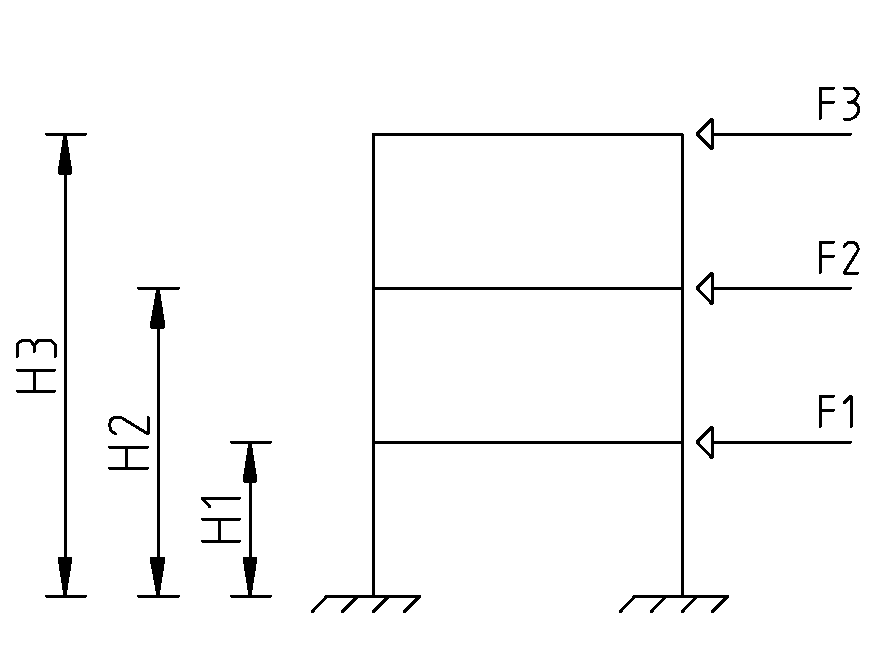
\includegraphics[width=0.5\textwidth]{Coeficiente-gamma-z/Imagens/M1-total-d.png}
	\end{center}
\end{figure}

Com isso,é possível verificar o deslocamento horizontal máximo permitido pela NBR 6118 - tabela 13.3. No topo é $H/1700$ e entre pavimentos é $H_{pisos}/850$, adotando-se coeficiente de pressão dinâmica do vento para cálculo do estado limite $\psi_1=0,30$.